
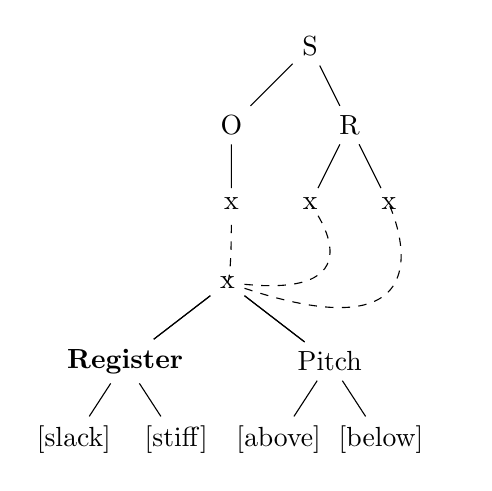
\begin{tikzpicture}
	\node (tbu) at (1.95,0) {x};
	\node (R) at (.65,-1) {\textbf{Register}};
	\node (P) at (3.25,-1) {Pitch};
	\node (r1) at (0,-2) {[slack]};
	\node (r2) at (1.3,-2) {[stiff]};
	\node (p1) at (2.6,-2) {[above]};
	\node (p2) at (3.9,-2) {[below]};
	\draw (tbu) -> (R) -> (r1);
	\draw (tbu) -> (R) -> (r2);
	\draw (tbu) -> (P) -> (p1);
	\draw (tbu) -> (P) -> (p2);
	% Second graph (shifted right)
	\begin{scope}[xshift=3cm, yshift=3cm]
		\node (sS) at (0,0) {S};
		\node (o) at (-1,-1) {O};
		\node (r) at (0.5,-1) {R};
		\node (x1) at (-1,-2) {x};
		\node (x2) at (0,-2) {x};
		\node (x3) at (1,-2) {x};
		\draw (sS) -> (o) -> (x1);
		\draw (sS) -> (r) -> (x2);
		\draw (r) -> (x3);
	\end{scope}
	
	% Cross edges from TBU to Xs
	\draw[dashed] (tbu) .. controls +(0,0) and +(0,-1) .. (x1);
	\draw[dashed] (tbu) .. controls +(2,-0.2) and +(0,0) .. (x2);
	\draw[dashed] (tbu) .. controls +(3,-1) and +(0,0) .. (x3);
\end{tikzpicture}\hfill
\begin{tikzpicture}[
	->, 
	node distance=1cm, 
	every node/.style={circle, draw, inner sep=2pt}, 
	re/.style={draw, rectangle, inner sep=2pt}
	]
	
	% top nodes
	\node (sS) {S};
	\node (o) [below left=0.5cm and 0.3cm of sS] {O};
	\node (r) [below right=0.5cm and 0.3cm of sS] {R};
	
	% skeletal tier
	\node (x1) [below=0.5cm of o] {x};
	\node (x2) [right=0.5cm of x1] {x};
	\node (x3) [right=0.5cm of x2] {x};
	\coordinate (left)  at ($(x1)+(-.5,0)$);
	\coordinate (right) at ($(x3)+(.5,0)$);
	
	% REGISTER tier
	\node (reg1) [below left =0.5cm of x1] {+st};
	\node (reg2) [below left =0.5cm of x2] {-sl};
	\node (reg3) [below left =0.5cm of x3] {+st};
	
	% PITCH tier
	\node (pit1) [below right =0.5cm and 0.5cm of reg3] {};
	\node (pit2) [right =0.5cm of pit1] {L};
	\node (pit3) [right =0.5cm of pit2] {H};
	
	% background dotted edge (drawn underneath everything else)
	
	
	% connections
	\draw (sS) -> (o);
	\draw (sS) -> (r);
	\draw (o) -> (x1);
	\draw (r) -> (x2);
	\draw (r) -> (x3);
	\draw (left) -> (x1);
	\draw (x1) -> (x2);
	\draw (x2) -> (x3);
	\draw (x3) -> (right);
	
	% associations
	\draw (x1) -> (reg1);
	\draw[dotted] (x2) -> (reg2);
	\draw[dotted] (x3) -> (reg3);
	\draw (x2) -> (pit2);
	\draw (x3) -> (pit3);
	
	% curved tier connections with labels
	
	\draw (pit2)to[out=-30,in=-150] (pit3);
	
	
	\draw (reg1)to[out=-30,in=-150] (reg2);
	\draw (reg2)to[out=-30,in=-150] (reg3);
	
\end{tikzpicture}

